\section{My Current Work}
\frame{\tableofcontents[currentsection, hideothersubsections]}

\begin{frame}
\frametitle{My current work: Interest}

\begin{figure}
    \centering
    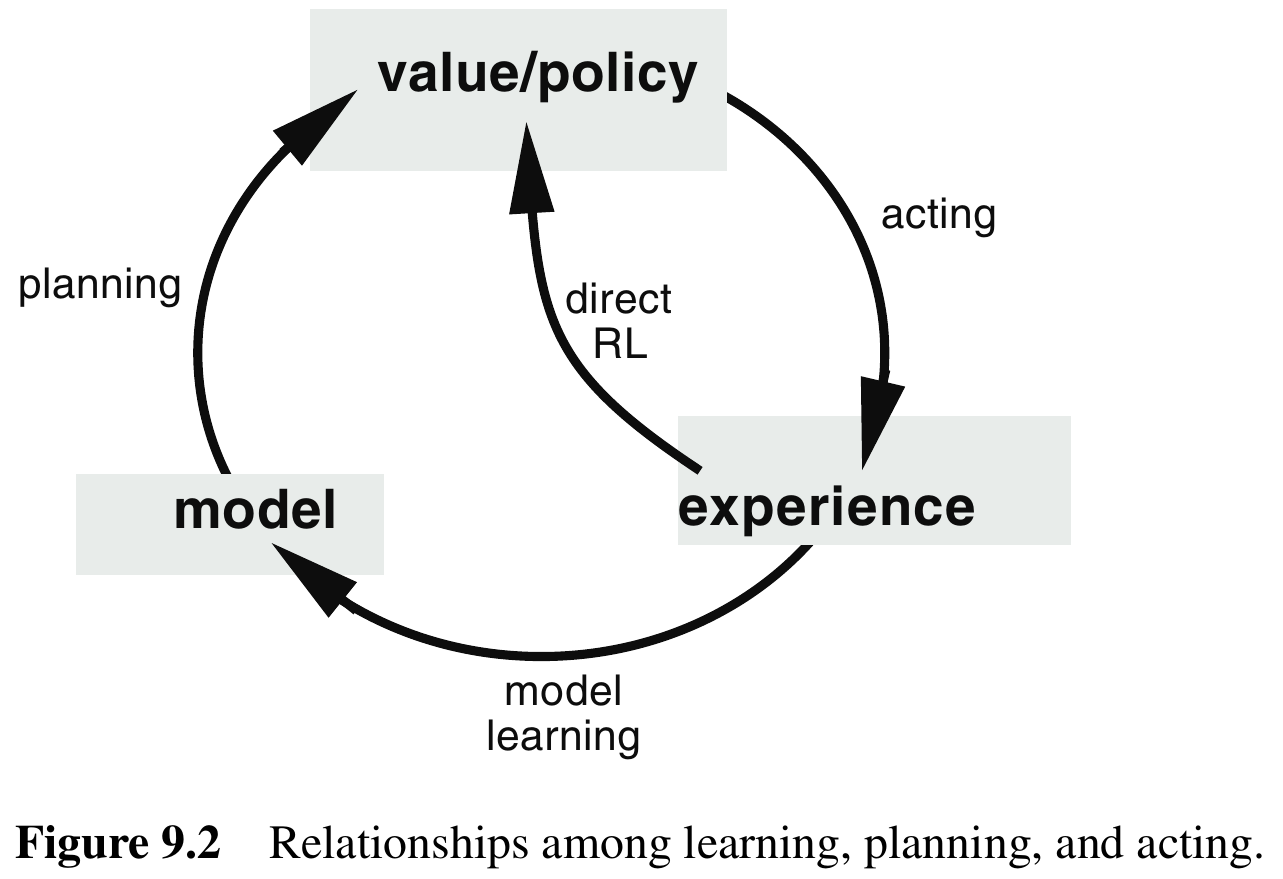
\includegraphics[scale=0.20]{learningplanning_arch}
\end{figure}

Interests, lack of ideas still :(
\begin{itemize}
  \item interaction of model-based and model-free RL, continuous control,
  deeply bayesian RL for POMDPs,
  \item physics-intensive tasks with real robots
\end{itemize}
\end{frame}

\begin{frame}
\frametitle{My current work: On going}
\begin{itemize}
  \item playing around with sim timestep, case: grasping
  \item movodemo, case: pickandplace
\end{itemize}
\vspace{5mm}

Enjoy: some videos!
\end{frame}

% \begin{frame}
% \frametitle{Interests: more detail}
% Nuts and Bolts Task:
% Assumed that the robot has already been trained to recognize, want, grasp, and eat cookies.
% The cookies in this task are within cages, and the cage covers are locked with nuts and bolts.
% The robot must learn to use a wrench and his fingers to remove the cover and get the cookie.
% \end{frame}

% Practical :
% \begin{itemize}
%   \item grasping, using tools,
%   e.g.  Nuts and Bolts Task:
%   \item navigation among movable obstacles
%   (motion planning with minimal collisions)
%   \item (physics) games, e.g
%   car racing, block stacking (simplified Tummple, Jenga)
% \end{itemize}
